%-------------------------------------------------------------------------------------------
\documentclass[aspectratio=169,UTF8,11pt]{ctexbeamer}

%%%%%%%%%%%%%%%%%%%%%%%%%%%%%
\usepackage{colortbl}
\usepackage{color}
\usepackage{booktabs}
\usepackage{threeparttable}
\usepackage{hyperref}
\usepackage{bm}
\usepackage{amsmath}
\usepackage[ruled,vlined]{algorithm2e}
%\usepackage{babel}
%%%%%%%%%%%%%%%%%%%%%%%%%%%%%

\mode<presentation> {
\usetheme{Madrid}
%\setbeamertemplate{footline} % To remove the footer line in all slides uncomment this line
\setbeamertemplate{footline}[frame number] % To replace the footer line in all slides with a simple slide count uncomment this line
\setbeamercolor{page number in head/foot}{fg=blue}
\setbeamertemplate{navigation symbols}{} % To remove the navigation symbols from the bottom of all slides uncomment this line
}

% User Defined Block %%%%%%%%%%%%%%%%%%%%%%%%%%%%%%%%%%%%%%%%%%%%%%%%%%%%%%%%
\usepackage{setspace}
\definecolor{orange}{rgb}{1,0.5,0}
\definecolor{aa}{RGB}{34,139,34}
\definecolor{lightblue}{rgb}{0,0.85,0.9}
\definecolor{darkblue}{rgb}{0,0.7,1}

\definecolor{hanblue}{rgb}{0.27, 0.42, 0.81}
\definecolor{indiagreen}{rgb}{0.07, 0.53, 0.03}
\definecolor{indianred}{rgb}{0.8, 0.36, 0.36}
\definecolor{indianyellow}{rgb}{0.89, 0.66, 0.34}
\definecolor{babypink}{rgb}{0.96, 0.76, 0.76}
\definecolor{ao(english)}{rgb}{0.0, 0.5, 0.0}
\setbeamerfont{block title}{size=\normalsize}
\setbeamerfont{block body}{size=\small}

\newenvironment<>{blueblock}[1]{%
  \setbeamercolor{block title}{fg=white,bg=hanblue}%
  \begin{block}#2{#1}}{\end{block}}

\newenvironment<>{greenblock}[1]{%
  \setstretch{1.3}\setbeamercolor{block title}{fg=white,bg=indiagreen}%
  \begin{block}#2{#1}}{\end{block}}

\newenvironment<>{redblock}[1]{%
  \setstretch{1.3}\setbeamercolor{block title}{fg=white,bg=indianred}%
  \begin{block}#2{#1}}{\end{block}}

\newenvironment<>{yellowblock}[1]{%
  \setstretch{1.3}\setbeamercolor{block title}{fg=white,bg=indianyellow}%
  \begin{block}#2{#1}}{\end{block}}

%----------------------------------------------------------------------------------------
%	PACKAGES
%----------------------------------------------------------------------------------------
\usepackage{graphicx} % Allows including images
%\usepackage{tikz}
%\usetikzlibrary{shapes.geometric, arrows}
\usepackage{listings}
\lstset{language=C++,
    columns=flexible,
   % basicstyle=\scriptsize\ttfamily,                                      % 设定代码字体、大小4
    basicstyle=\footnotesize\ttfamily,
    %numbers=left,xleftmargin=2em,framexleftmargin=2em,                   % 在左侧显示行号
    %numberstyle=\color{darkgray},                                        % 设定行号格式
    keywordstyle=\color{blue},                                            % 设定关键字格式
    commentstyle=\color{ao(english)},                                     % 设置代码注释的格式
    stringstyle=\color{brown},                                            % 设置字符串格式
    %showstringspaces=false,                                              % 控制是否显示空格
	%frame=lines,                                                         % 控制外框
    breaklines,                                                           % 控制是否折行
    postbreak=\space,                                                     % 控制折行后显示的标识字符
    breakindent=5pt,                                                      % 控制折行后缩进数量
    emph={size\_t,array,deque,list,map,queue,set,stack,vector,string,pair,tuple}, % 非内置类型
    emphstyle={\color{teal}},
    escapeinside={(*@}{@*)},
}
%---------------------------------------------------------------------------------------------------

%%%%%%%%%%%%%%%%%%%%%%%%%%%%%%%%%%%%%%%%%%%%%%%%%%%%%%%%%%%%%%%%%%%%%%%%%%%%%%%%%%%%%%%%%%%%%%
\title[\textit{智能优化与最优化方法}]{15.4 Games}
\author[李长河]{李长河} % Your name
\institute[CUG] % Your institution as it will appear on the bottom of every slide, may be shorthand to save space
{
中国地质大学(武汉)自动化学院\\ % Your institution for the title page
\medskip
\textit{lichanghe@cug.edu.cn} % Your email address
}
\date{} % Date, can be changed to a custom date
%%%%%%%%%%%%%%%%%%%%%%%%%%%%%%%%%%%%%%%%%%%%%%%%%%%%%%%%%%%%%%%%%%%%%%%%%%%%%%%%%%%%%%%%%%%%%%

\usefonttheme[onlymath]{serif}
\begin{document}
\maketitle
\begin{frame}[noframenumbering]           %beamer里重要的概念,每个frame定义一张page
\centering
{\large 李长河 \vspace{0.5cm} \\自动化学院710 \vspace{0.5cm}\\ lichanghe@cug.edu.cn}
\end{frame}

%-----------------------------------------------------------


\addtocounter{framenumber}{-1}
%---------------------------------------------------------------------------------------------

\begin{frame}{Contents}
	\tableofcontents
\end{frame}

%%%%%%%%%%%%%%%%%%%%%%%%%%%%%%%%%%%%%%%%%%%%%%%%%%%%%%%%%%%%%%%%%%%%%%%%%%%%%%%%%%%%%%%%%%%%%%
\section{15.4 Games}
\begin{frame}
  {Games}
  \begin{block}{}
    For AI research, researchers attempt to devise computational systems that would exhibit aspects of \alert{human intelligence} and achieve \alert{human-level} problem solving or decision making abilities.
  \end{block}
  \begin{block}{}
    The highly formalized, symbolic representation allowed AI to success in many cases.
  \end{block}
  \begin{greenblock}{}
    Naturally, games, especially board games, have been a popular domain for AI researches as they are \alert{formal} and \alert{highly constrained}, yet \alert{complex}, decision making environments. 
  \end{greenblock}
\end{frame}

%%%%%%%%%%%%%%%%%%%%%%%%%%%%%%%%%%%%%%%%%%%%%%%%%%%%%%%%%%%%%%%%%%%%%%%%%%%%%%%%%%%%%%%%%%%%%%
\subsection{15.4.1 Applications}
\begin{frame}
  \tableofcontents[currentsection,currentsubsection]
\end{frame}

\begin{frame}
  {Games\small{-Applications}}
  \begin{yellowblock}{}
    There are two main applications of intelligent optimization on games:
    \begin{itemize}
      \item Game playing
      \item Content generation
    \end{itemize}
  \end{yellowblock}
\end{frame}

\begin{frame}
  {Games\small{-Applications}}
  \begin{block}{Game Playing}
    For game playing, there are two main ways to use the intelligent optimization:
    \begin{itemize}
      \item Offline optimization: Optimizing the parameters of a pre-defined controller, then using the optimized controller to play the game.
      \item Online optimization (or evolutionary planning): Optimizing the actions to be deployed while the game is running.
    \end{itemize}
  \end{block}
\end{frame}

\begin{frame}
  {Games\small{-Applications}}
  \begin{block}{In the offline optimization}
    The intelligent optimization algorithm can be combined with many other methods. In particular, using EAs to evolve: 
    \begin{itemize}
      \item the weights and/or topology of \alert{neural networks}, 
      \item or \alert{programs}, typically structured as expression trees (e.g., genetic programming), 
      \item or some other \alert{models}, such as potential field.
    \end{itemize}
    This fitness evaluation consists of using the neural network, program or other models to play the game, and using the \alert{result (e.g., score) as a fitness function}.
  \end{block}
\end{frame}

\begin{frame}
  {Games\small{-Applications}}
  \begin{block}{In the online optimization}
    The basic idea is to optimize the \alert{action sequence} you want to deploy from now on. Evaluating such an action sequence is done by taking all the actions of the sequence in \alert{simulation}, and observing the results after taking all those actions.
  \end{block}
  \begin{block}{}
    The online optimization has been applied on several types of games such as: 
    \begin{itemize}
      \item arcade game
      \item turn-based strategy game
      \item real-time strategy game
    \end{itemize}
  \end{block}
\end{frame}

\begin{frame}
  {Games\small{-Applications}}
  \begin{block}{Content Generation}
    Procedural content generation refers to the methods which generate game content either automatically or with only limited human input, such as: 
    \begin{itemize}
      \item levels
      \item maps
      \item game rules
    \end{itemize}
  \end{block}
  \begin{blueblock}{}
    The search-based methods are widely used in this area because we will eventually get the solution we want if we keep iterating and tweaking solutions by keeping the good changes and discarding the bad changes. 
  \end{blueblock}
\end{frame}
%%%%%%%%%%%%%%%%%%%%%%%%%%%%%%%%%%%%%%%%%%%%%%%%%%%%%%%%%%%%%%%%%%%%%%%%%%%%%%%%%%%%%%%%%%%%%%
\subsection{15.4.2 A Simple Example of Real-time Strategy Game}
\begin{frame}
  \tableofcontents[currentsection,currentsubsection]
\end{frame}

\begin{frame}
  {Games\small{-A Simple Example of Real-time Strategy Game}}
  \begin{block}{A simple online optimization example}
    Playing a simple scene in a famous real-time strategy (RTS) game: StarCraft II
  \end{block}
  \begin{block}{}
    The features of a RTS game bring some challenges for AI research, including: 
    \begin{itemize}
      \item Incomplete information
      \item Long term planning
      \item Large search space
      \item Real time
    \end{itemize}
  \end{block}
\end{frame}

\begin{frame}
  {Games\small{-A Simple Example of Real-time Strategy Game}}
  \begin{columns}[T]
    \column{0.5\textwidth}
    \begin{block}{Scenario Settings}
      The figure presents an example map for a game scenario: 
    \end{block}
    \begin{block}{Components}
      \begin{itemize}
        \item Three Thors and one Marine in our team
        \item Some Auto-turrets in the enemy team
        \item Some toxic areas in the middle of the map, which will harm our units
      \end{itemize}
    \end{block}
  \column{0.4\textwidth}
  \begin{figure}[h]
    \centering
    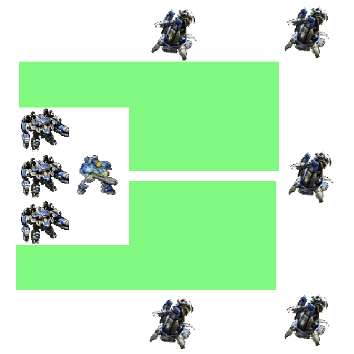
\includegraphics[width=0.5\textwidth,height=0.5\textwidth]{fig15-4-TvsA.pdf}
    \caption{An example map: Auto-turrets vs Thors and a Marine, where toxic areas are indicated in green}
    \label{fig15-4-AvsT}
    \end{figure}
  \end{columns}
  \begin{blueblock}{}
    The focus of this scenario is to test whether the algorithm can find and maintain reasonable tactical positions for different units. 
  \end{blueblock}
\end{frame}

\begin{frame}
  {Games\small{-A Simple Example of Real-time Strategy Game}}
  \begin{block}{A Multi-objective Approach}
    \begin{itemize}
      \item The algorithm runs in the online mode within a given time during the game.
      \item A solution is selected and deployed when the running time is over. 
    \end{itemize}
  \end{block}
  \begin{block}{Components}
    \begin{itemize}
      \item Solution representation
      \item Problem representation
      \item Evaluation
      \item Selection
    \end{itemize}
  \end{block}
\end{frame}

\begin{frame}
  {Games\small{-A Simple Example of Real-time Strategy Game}}
  \begin{block}{Solution representation}
    A solution contains the sequence of actions to be performed by all units in the next period of time.
  \end{block}
  \begin{block}{}
    Suppose we have $M$ units, and each unit has $C$ actions, then the $j$-th action of the $i$-th unit can be represented as $a_{ij}$, $i\in\{1,2,\dots,M\}$, $j\in\{1,2,\dots,C\}$, then a solution $s$ can be represented as: 
    \begin{equation*}
      \bm x =
      \begin{pmatrix}
      a_{11} & a_{12} & \cdots & a_{1C} \\
      a_{21} & a_{22} & \cdots & a_{2C} \\
      \vdots & \vdots & \ddots & \vdots \\
      a_{M1} & a_{M2} & \cdots & a_{MC}
      \end{pmatrix}
      \end{equation*}
      where $a$ is a 2-tuple, i.e., $a=(actionId, targetPoint)$,  $actionId$ represents the action to be deployed and $targetPoint$ determines the target location of the action.
  \end{block}
  \begin{yellowblock}{}
    To simplify the problem, we only take the attack action into consideration.
  \end{yellowblock}
\end{frame}

\begin{frame}
  {Games\small{-A Simple Example of Real-time Strategy Game}}
  \begin{block}{Problem representation}
    The problem is transformed to a dynamic multi-objective optimization problem, which is shown below: 
  \end{block}
  \begin{block}{}
    where $t_0$ and $t$ denote the starting and ending time of a simulation; $M_t$ and $N_t$ denote the number of units of our team and the enemy team at simulation time $t$ ; $h_i$ and $s_i$ are the health points and shield of unit $i$;   $t^{end}$ is the loop at which the simulation ends when one team has been eliminated. 
  \end{block}
  \begin{block}{}
    \begin{align}
      \max f_1(x(t)) & = - (\sum_{i=1}^{M_t} (h_i(x(t_0)) + s_i(x(t_0)) - h_i(x(t)) - s_i(x(t))) \tag{1}   \\
      \max f_2(x(t)) & = \sum_{i=M_t+1}^{M_t+N_t}(h_i(x(t_0)) +s_i(x(t_0)) - h_i(x(t)) - s_i(x(t))) \tag{2}
      \end{align}
  \end{block}
  \begin{block}{}
    $f_1$ and $f_2$ are the damage of both teams during the simulation, respectively.
  \end{block}
\end{frame}

\begin{frame}
  {Games\small{-A Simple Example of Real-time Strategy Game}}
  \begin{block}{}
    where $t_0$ and $t$ denote the starting and ending time of a simulation; $M_t$ and $N_t$ denote the number of units of our team and the enemy team at simulation time $t$ ; $h_i$ and $s_i$ are the health points and shield of unit $i$;   $t^{end}$ is the loop at which the simulation ends when one team has been eliminated. 
  \end{block}
  \begin{block}{}
    \begin{align}
      \max f_3(x(t)) & =
      \begin{cases}
      -(t^{end}(x(t))-t_0)&\text{if win}\\ \tag{3}
      -(t-t_0) &\text{else}
      \end{cases}\\
      \max f_4(x(t)) &=
      \begin{array}{lr}
      \sum^{M_t+N_t}_{i=M_t+1}\left(\min_{i\le j \le M_t} \mathrm{Dis}\left(p_i(x(t_0)), p_j(x(t_0))\right) \right.- \tag{4}\\
       \left.\min_{1\le j\le M_t} \textrm{Dis}\left(p_i(x(t), p_j(x(t)))\right)\right)
      \end{array}
      \end{align}
  \end{block}
  \begin{block}{}
    $f_3$ is the duration of the game when any team is completely destroyed in the simulation; \\
    $f_4$ is used to guide our team to move to the target position, especially when our team can not get near enough to fight against the enemy during the simulation as $f_1, f_2, f_3$ can not obtain valid values (the values of $f_1, f_2, f_3$ for all solutions are the same of zero if no fight happens).
  \end{block}
\end{frame}

\begin{frame}
  {Games\small{-A Simple Example of Real-time Strategy Game}}
  \begin{block}{}
    Considering the importance of the four objectives, the more important objectives f1, f2, f3 could be used first to sort the solutions, then the f4.
  \end{block}
  \begin{yellowblock}{}
    So this model can be regarded as a two-level four-objective dynamic optimization problem.
  \end{yellowblock}
\end{frame}

\begin{frame}
  {Games\small{-A Simple Example of Real-time Strategy Game}}
  \begin{block}{Evaluation}
    A solution is evaluated through the simulation. 
  \end{block}
  \begin{yellowblock}{}
    The debug interface of SC2API can be used to call other game processes running simultaneously to copy the current state and the orders in the solution then forward the game to a certain period.
  \end{yellowblock}
\end{frame}

\begin{frame}
  {Games\small{-A Simple Example of Real-time Strategy Game}}
  \begin{block}{}
    After the evolutionary search, a set of non-dominated solutions may be obtained. However, only one of the solutions  $\tilde{x}(t)$ at time will be selected and deployed. A rule-based method is used for the decision-making. 
  \end{block}
  \begin{block}{Selection}
    he solution is selected based on the current total points of both team: 
  \end{block}
  \begin{block}{}
    \begin{align}
      \tilde{x}(t)=\, & \arg \max_{x(t)} (\frac{f_1(x(t))}{\sum_{i=1}^{M_{t_0}}(h_i(x(t_0))+s_i(x(t_0)))} + \frac{f_2(x(t))} {\sum^{M_{t_0}+N_{t_0}}_{i=M_{t_0}+1}(h_i(x(t_0))+s_i(x(t_0))}) \tag{5}
      \end{align}
  \end{block}
\end{frame}

\begin{frame}
  {Games\small{-A Simple Example of Real-time Strategy Game}}
  \begin{block}{Results and Discussions}
    The algorithm can led our Thors approach the enemies along a narrow security area then stand outside the enemies’ fire range to attack them. The only Marine roams outside the enemies’ fire range.
  \end{block}
  \begin{columns}[T]
    \column{0.6\textwidth}
    \begin{figure}[width=0.3\textwidth,height=0.3\textwidth]
      \centering
      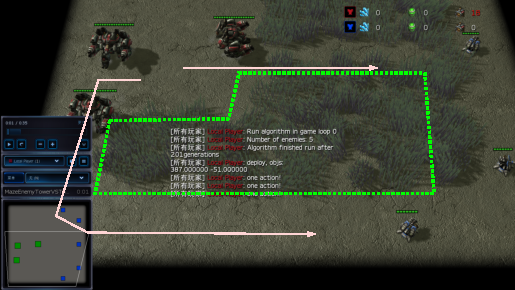
\includegraphics{fig15-4-x-gameshot}
      % \caption{Screenshot in the game}
    \end{figure}
    \column{0.35\textwidth}
    \begin{greenblock}{Results and Discussions}
      The algorithm can led our Thors approach the enemies along a narrow security area then stand outside the enemies’ fire range to attack them.
    \end{greenblock}
  \end{columns}
\end{frame}

\begin{frame}
  {Games\small{-A Simple Example of Real-time Strategy Game}}
  \begin{block}{}
    This is just a simple example with some static enemies.
  \end{block}
  \begin{block}{Results and Discussions}
    \begin{itemize}
      \item When there are movable enemies, it needs to handle the uncertainty of the enemy strategy. 
      \item In terms of understanding the enemy, opponent modeling can help. 
      \item If the algorithm run without any priori knowledge, adversarial co-evolution could be a way to generate reasonable solutions.
      \item To make the solutions more robust, more adaptable for various scenario, robust optimization can be useful.
    \end{itemize}
  \end{block}
  \begin{yellowblock}{}
    A special algorithm with some problem-specific search operators, which takes correlation between units and actions into consideration rather than basic EAs, would be more effective in solving this problem.
  \end{yellowblock}
\end{frame}

\end{document}